\section{Supporting figures}

\begin{figure}
%\centering
\hspace{-2cm}
\begin{tabular}{cc}
  \begin{subfigure}[b]{0.48\textwidth}
  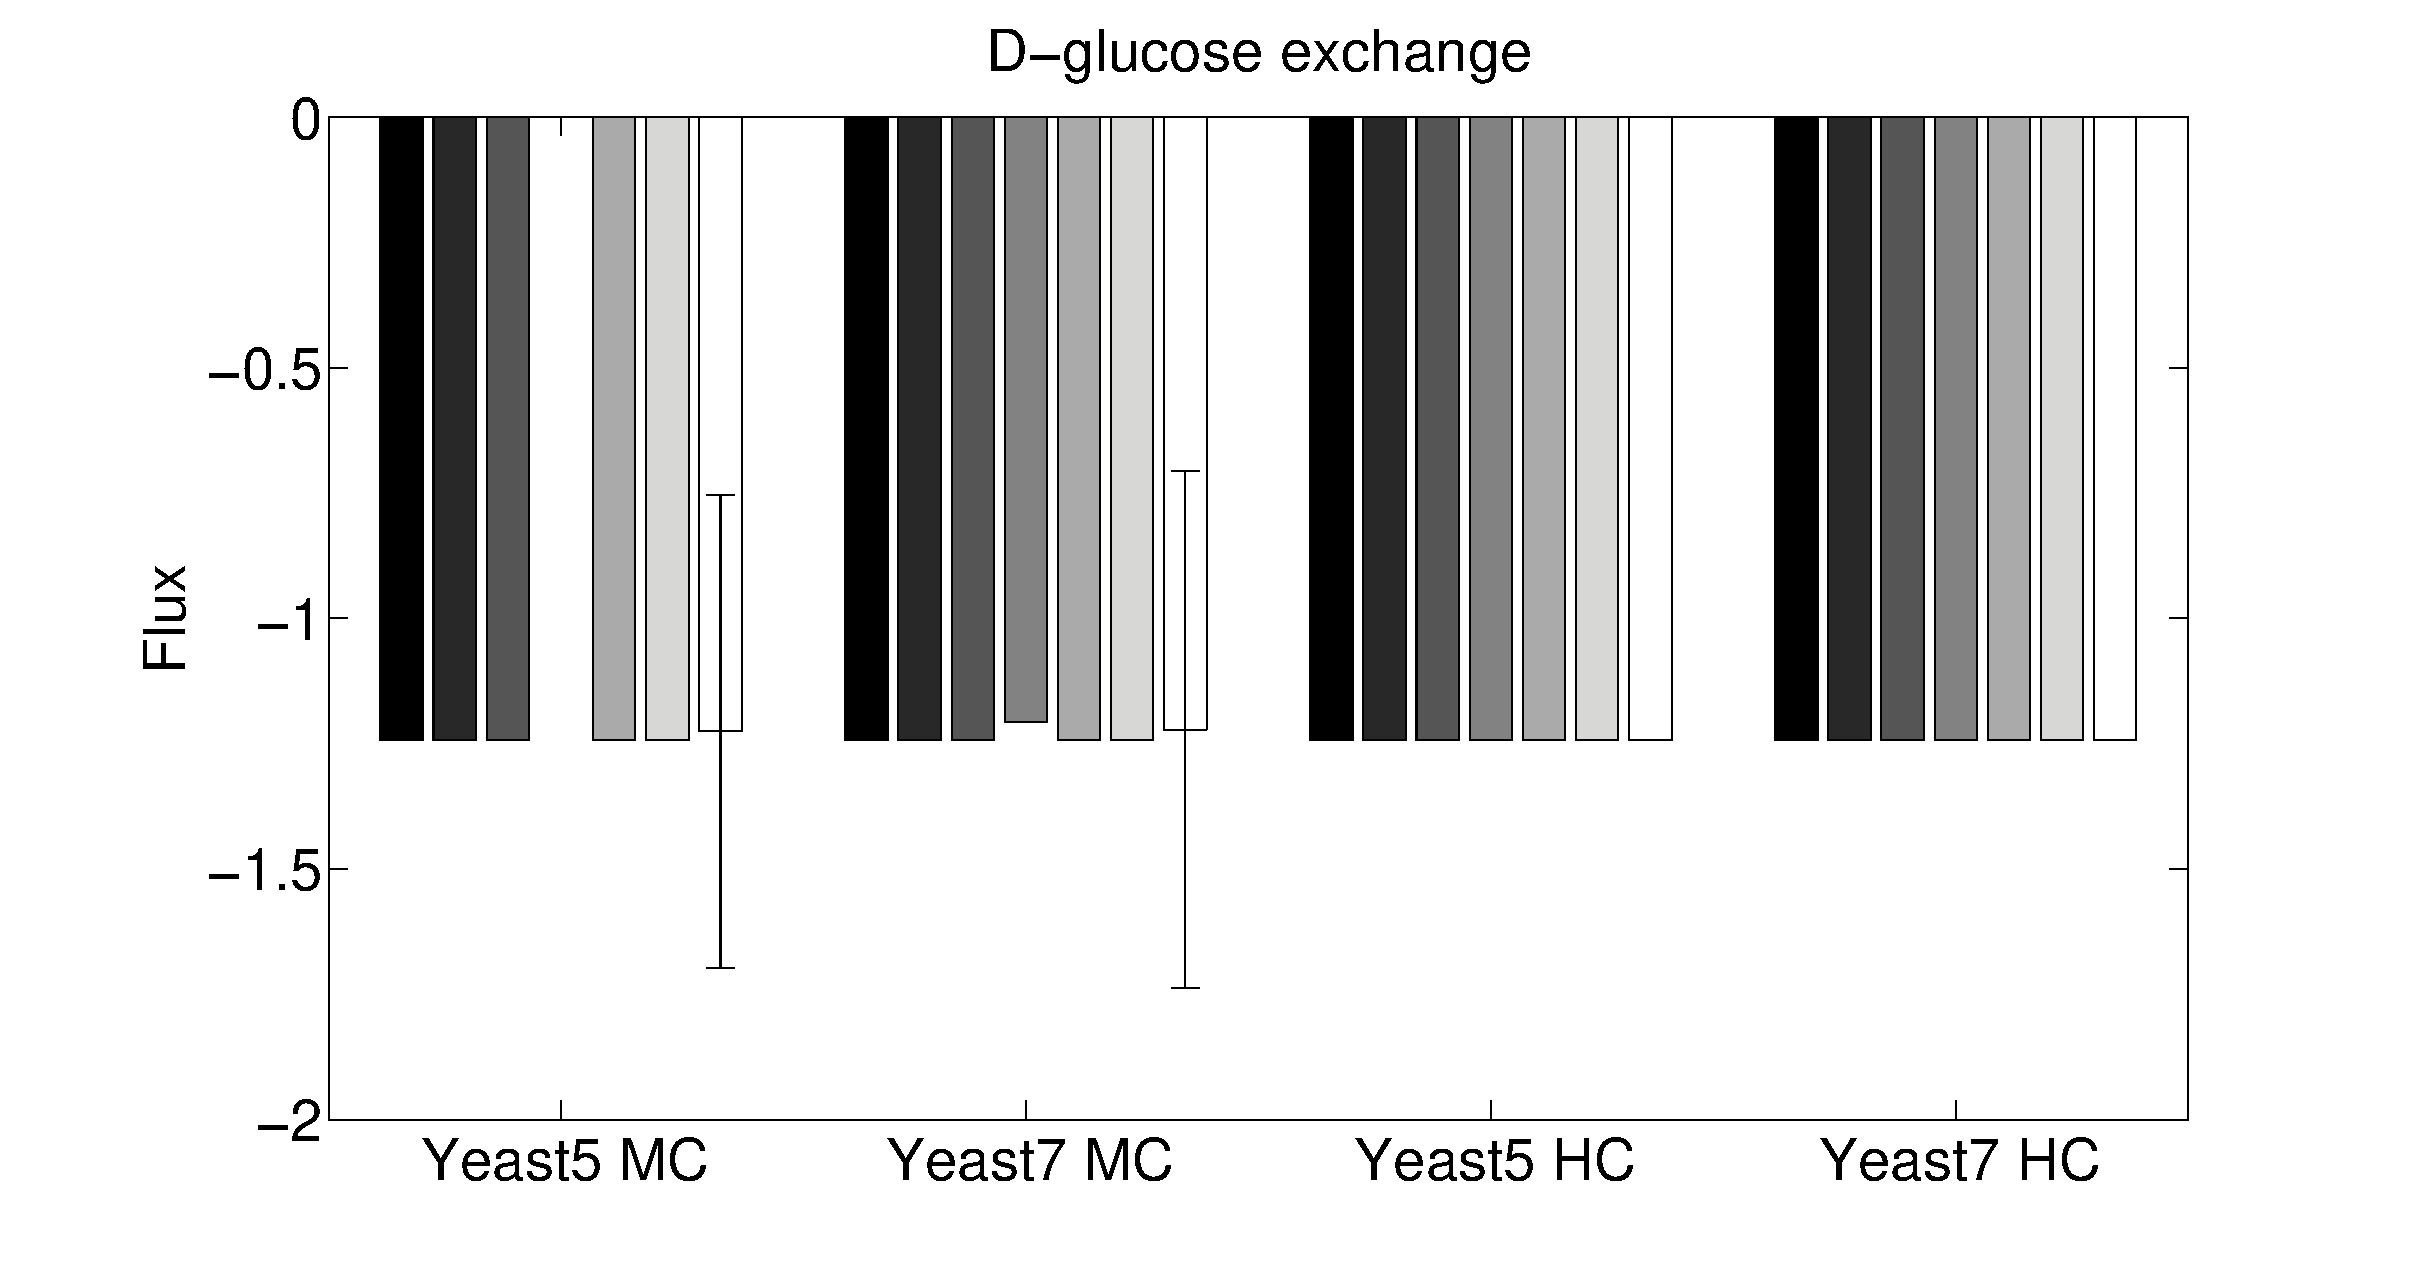
\includegraphics[width=\textwidth]{gluc75_bars}
  \end{subfigure}
&
  \begin{subfigure}[b]{0.48\textwidth}
  \hspace{2cm}
  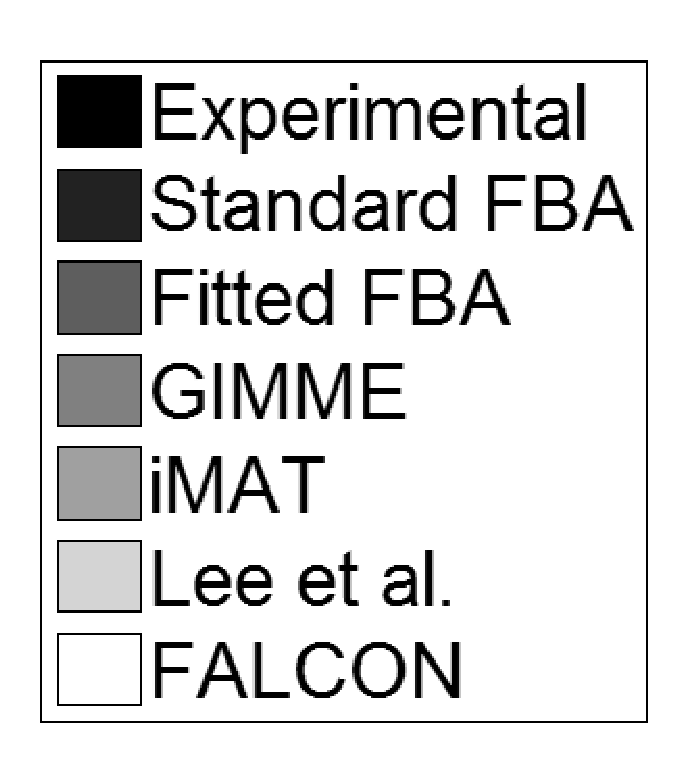
\includegraphics[scale=0.3,center]{legend_bars}
  \end{subfigure} 
\\
  \begin{subfigure}[b]{0.48\textwidth}
  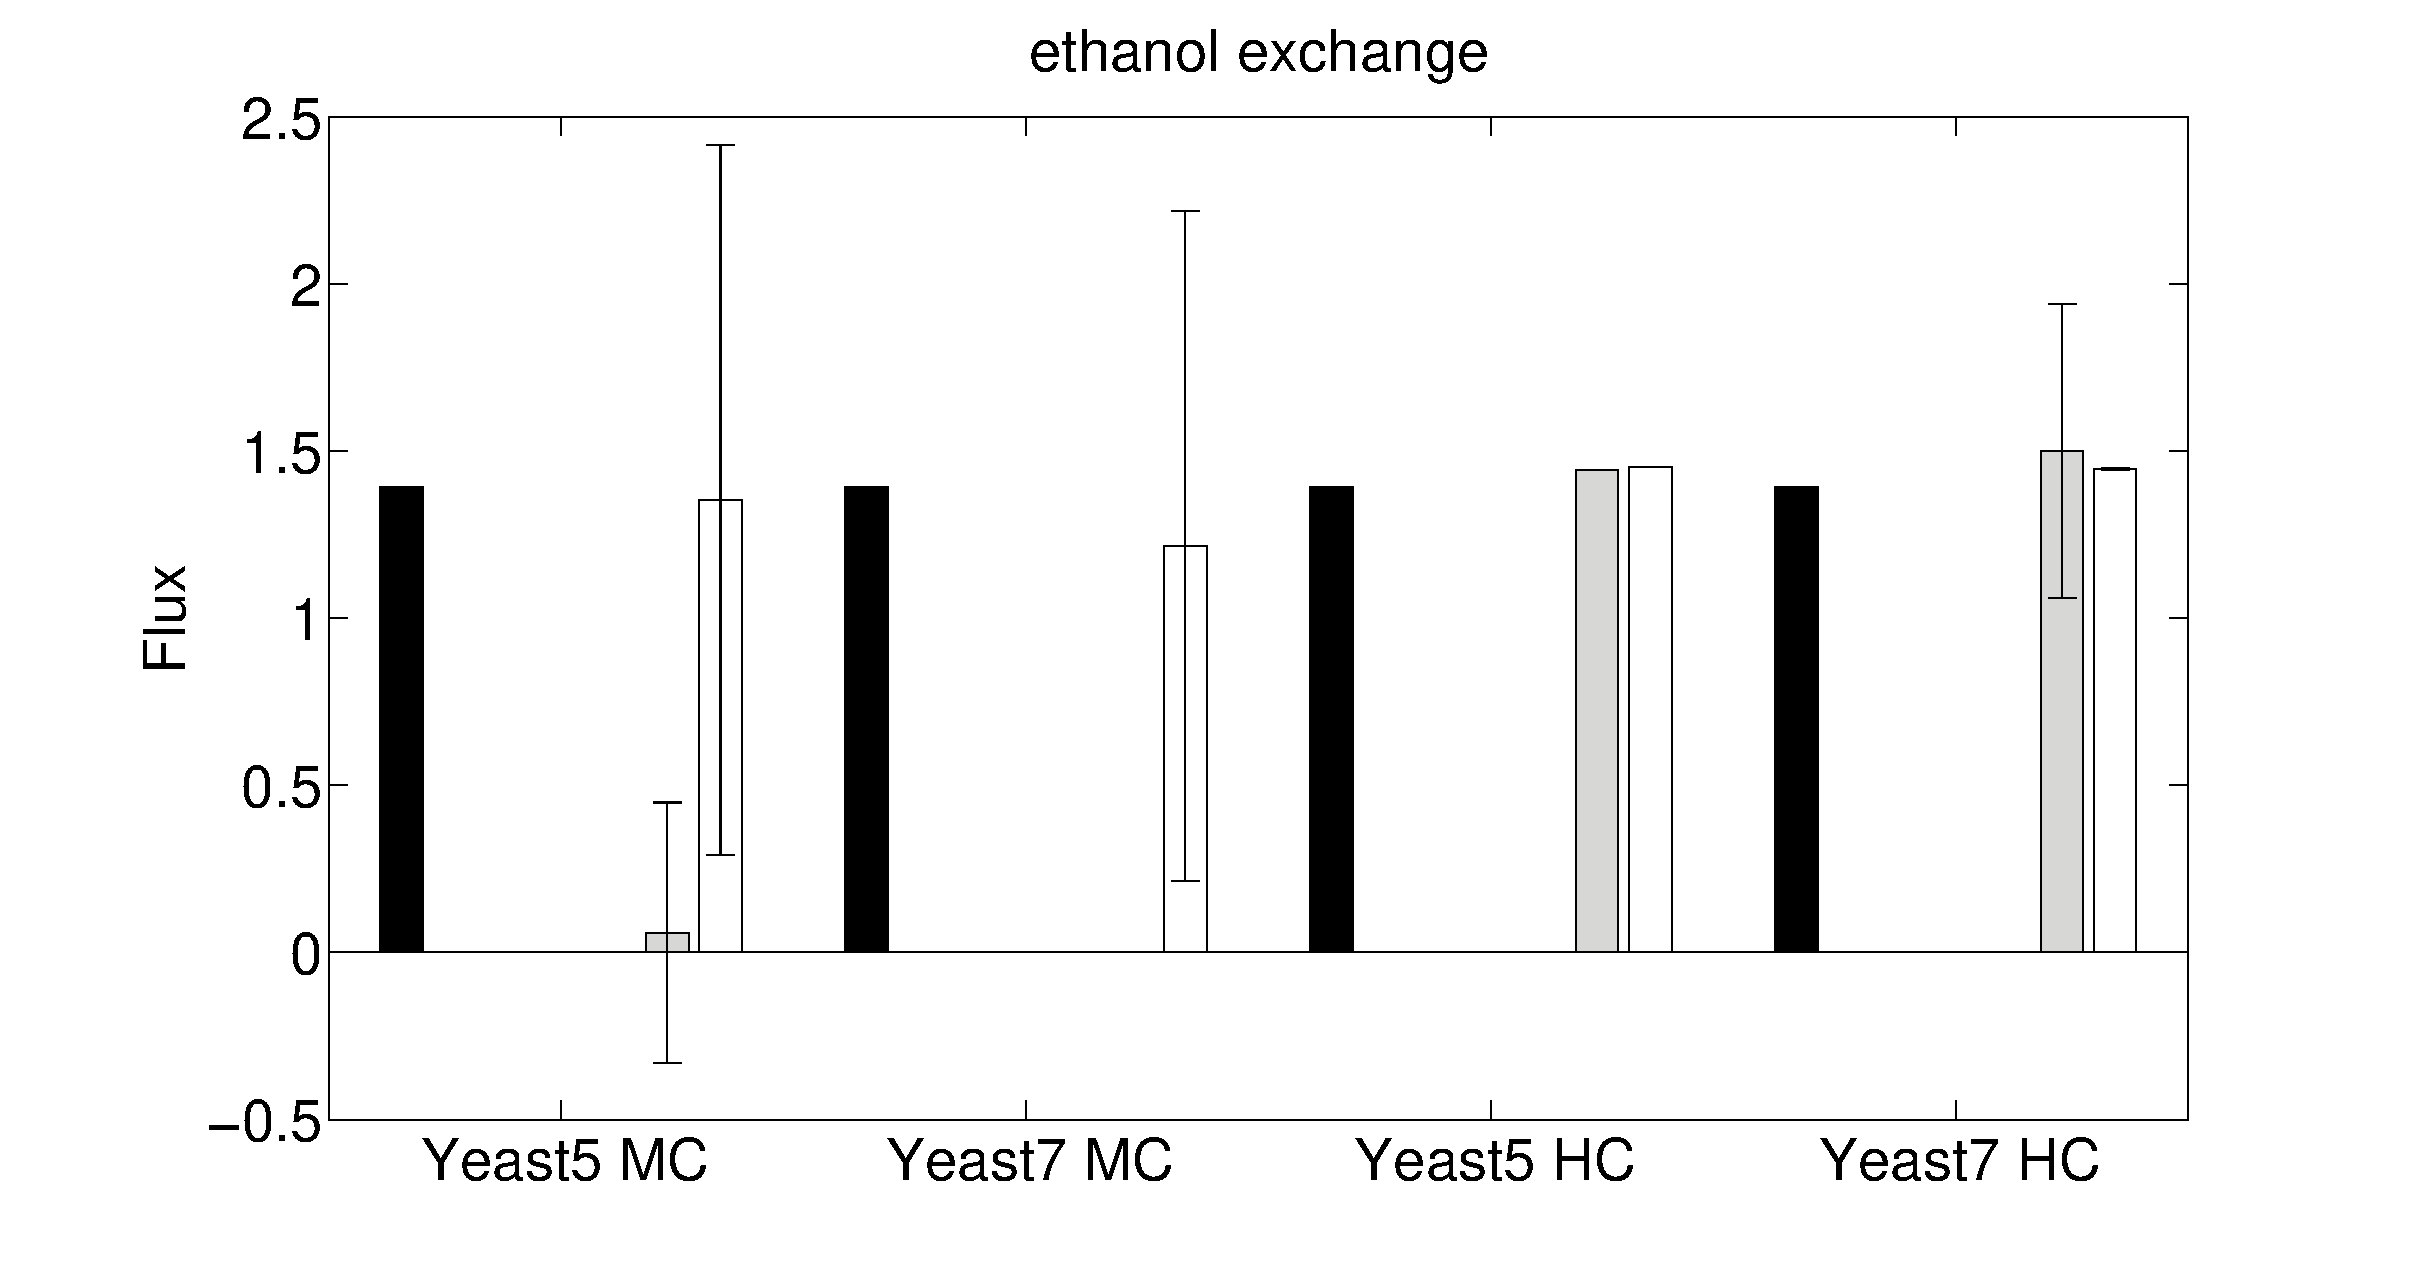
\includegraphics[width=\textwidth]{eth75_bars}
  \end{subfigure} 
&
  \begin{subfigure}[b]{0.48\textwidth}
  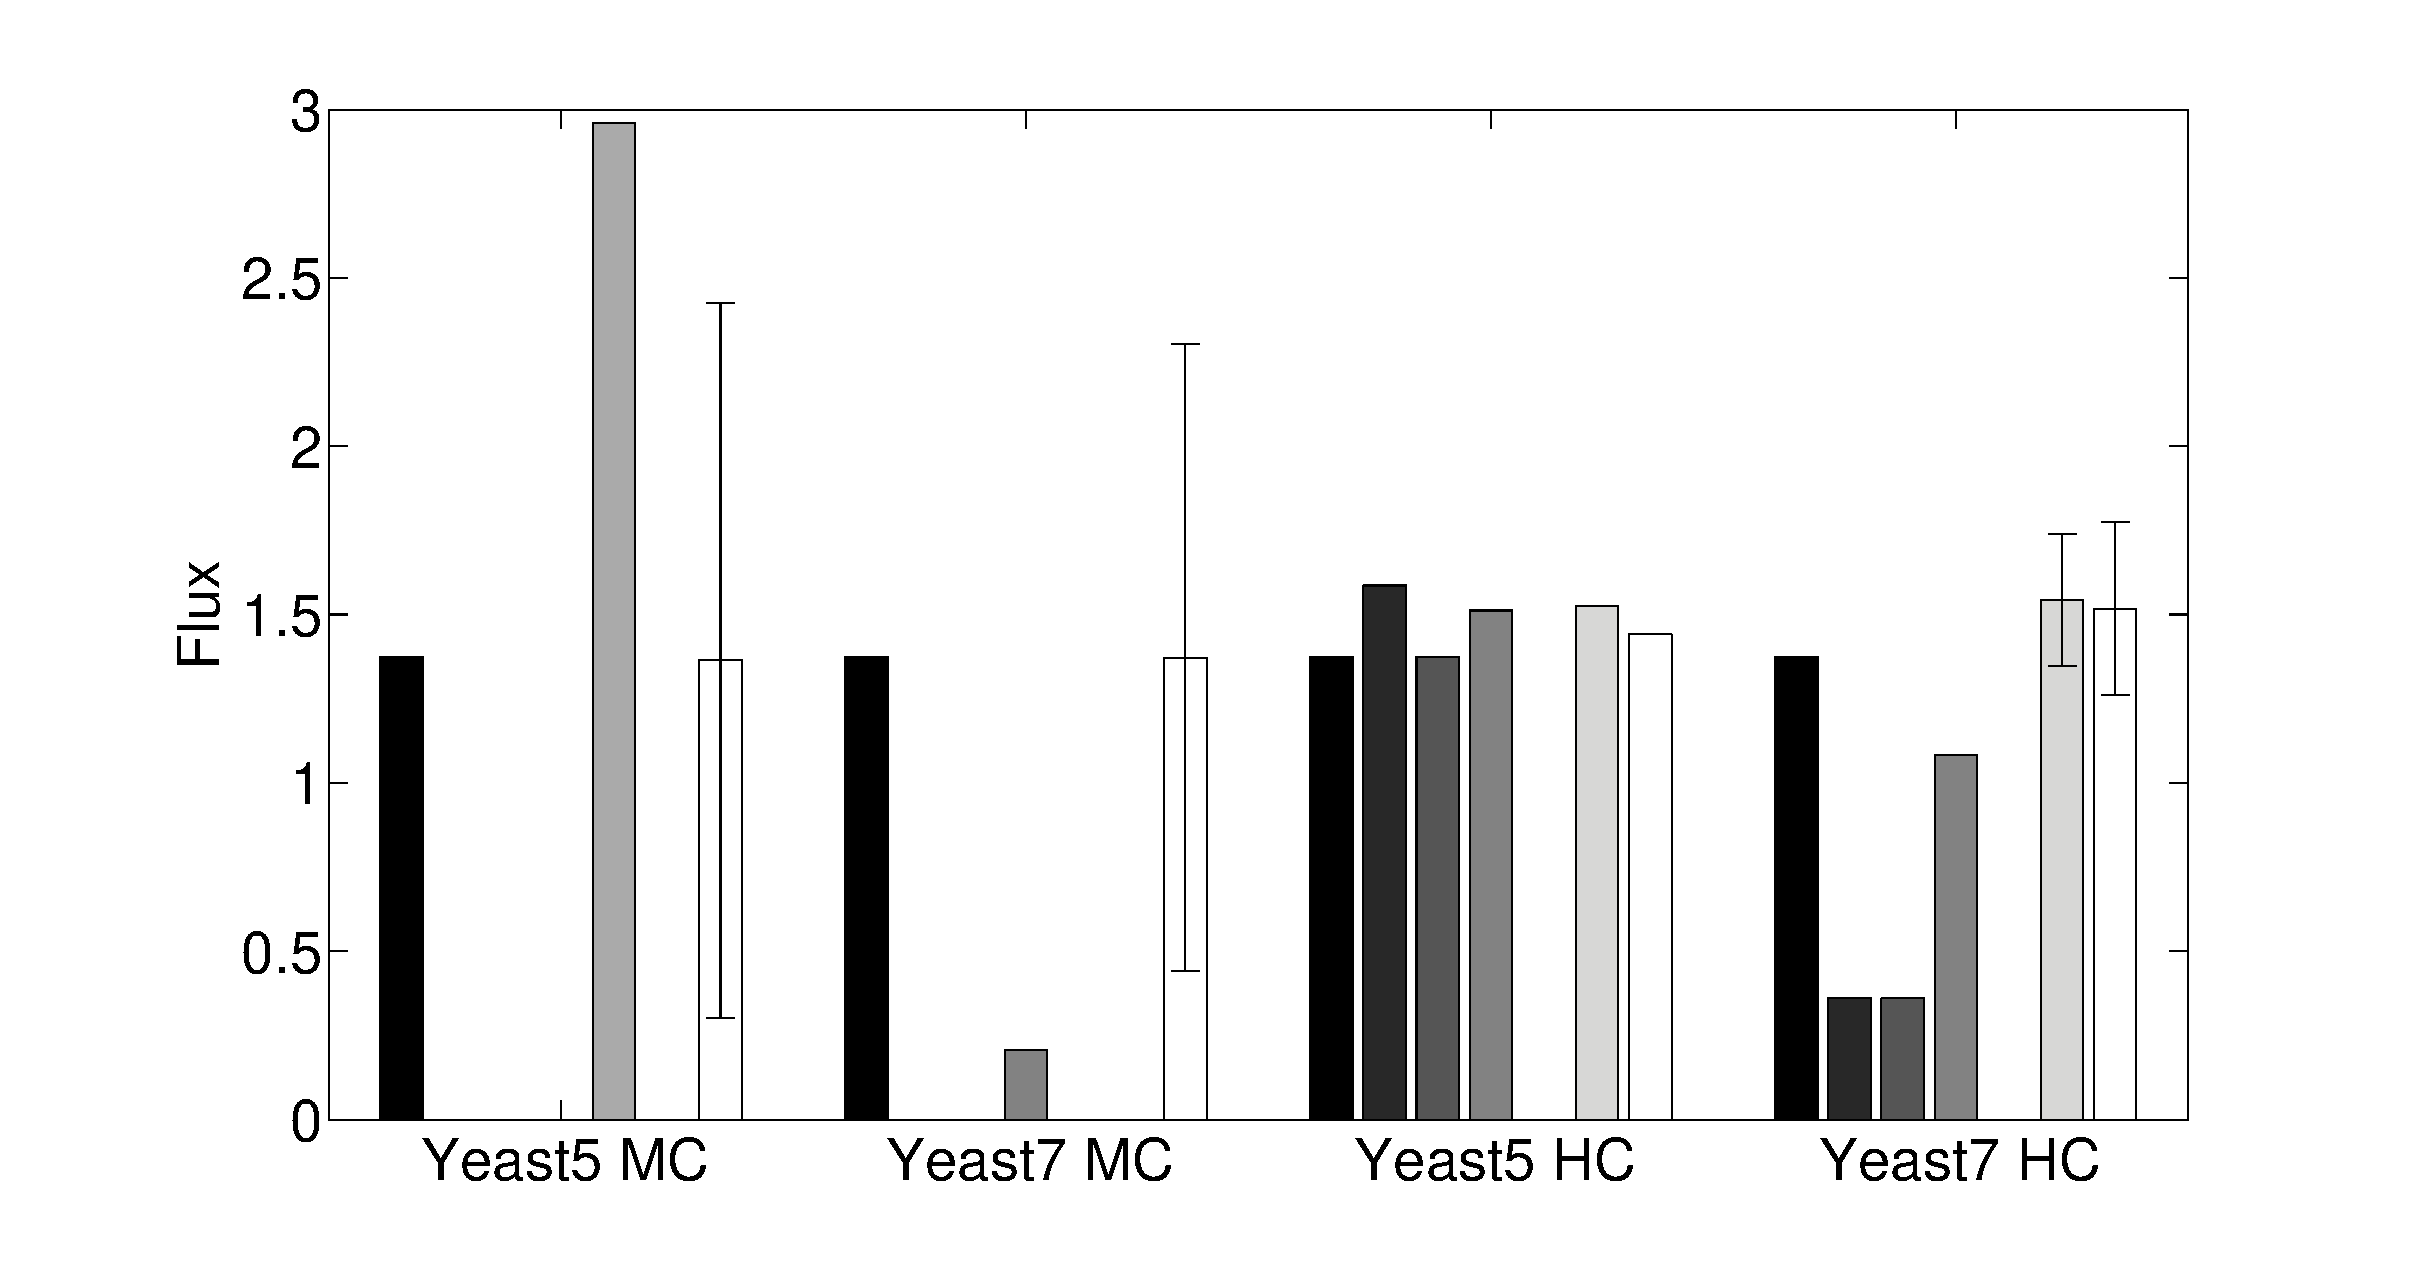
\includegraphics[width=\textwidth]{co2_75_bars}
  \end{subfigure} 
\\
\end{tabular}
\caption{
Shown are flux predictions using a number of methods and four
different models (Yeast5MC and Yeast7MC are minimally constrained
Yeast5 and Yeast7; Yeast5HC and Yeast7HC are highly constrained Yeast5
and Yeast7). Error bars are shown for the Lee et al. method and for
FALCON, where one side of the error bar corresponds to a standard
deviation. Note that there can be no variation for glucose in the
former case since glucose flux is fixed as part of the method. FALCON
performs very well for large fluxes (A-C), and is also the best
performer in general for the next largest flux, glycerol (D). It also
has sporadic success for smaller fluxes, but all methods seem to have
trouble with the smallest fluxes (e.g. E). Note that fluxes are drawn
in log scale (specifically a flux v is drawn as , sign(v) * log10(1 +
v)). Similar results are obtainable for the 85\% maximum growth
condition.}
\label{fig:FluxBars}
\end{figure}

\section{Assumptions for enzyme complex formation}
\label{sec:complexation}

In order to quantify enzyme complex formation (sometimes called enzyme
complexation), the notion of an enzyme complex should be formalized.
A protein complex typically refers to two or more physically
associated polypeptide chains, which is sometimes called a quaternary
structure. Since we are not exclusively dealing with multiprotein
complexes, we refer to an enzyme complex as being one or more
polypeptide chains that act together to carry out metabolic
catalysis.


\emph{Assumption~\ref{asm:expcorr}.}  A fundamental assumption
that we need in order to guarantee an accurate estimate of (unitless)
enzyme complex abundance are the availability of accurate measurements
of their component subunits. Unfortunately, this is currently not
possible, and we almost always must make do with mRNA measurements,
which may even have some degree of inaccuracy in measuring the mRNA
abundance. What has been seen is that Spearman's $\rho = 0.6$ for
correlation between RNA-Seq and protein intensity in datasets from
HeLa cells \citep{Nagaraj2011}. This implies that much can likely
still be gleamed from analyzing RNA-Seq data, but, an appropriate
degree of caution must be used in interpreting results based on
RNA-Seq data. By incorporating more information, such as metabolic
constraints, we hope to obviate some of the error in estimating
protein intensity from RNA-Seq data.

\emph{Assumption~\ref{asm:isozyme}.} We also include the notion of
isozymes--different proteins that catalyze the same reaction--in our
notion of enzyme complex. Isozymes may arise by having one or more
differing protein isoforms, and even though these isoforms may not be
present in the same complex at the same moment, we consider them to be
part of the enzyme complex since one could be substituted for the
other.

As an example for assumptions described so far, take the $F_1$
subcomplex of ATP Synthase (Figure~\ref{fig:2F43}), which is composed
of seven protein subunits (distinguished by color, left). On the
right-hand side we see different isoforms depicted as different
colors.  Error in expression data aside, instead of considering the
abundances with multiplicity and dividing their expression values by
their multiplicity, it may be easier to simply note that the axle
peptide (shown in red in the center of the complex) only has one copy
in the complex, so its expression should be an overall good estimation
of the $F_1$ subcomplex abundance. This reasoning will be useful
later in considering why GPR rules may be largely adequate for estimating
the abundance of most enzyme complexes.

\begin{figure*}%[H]
\centering
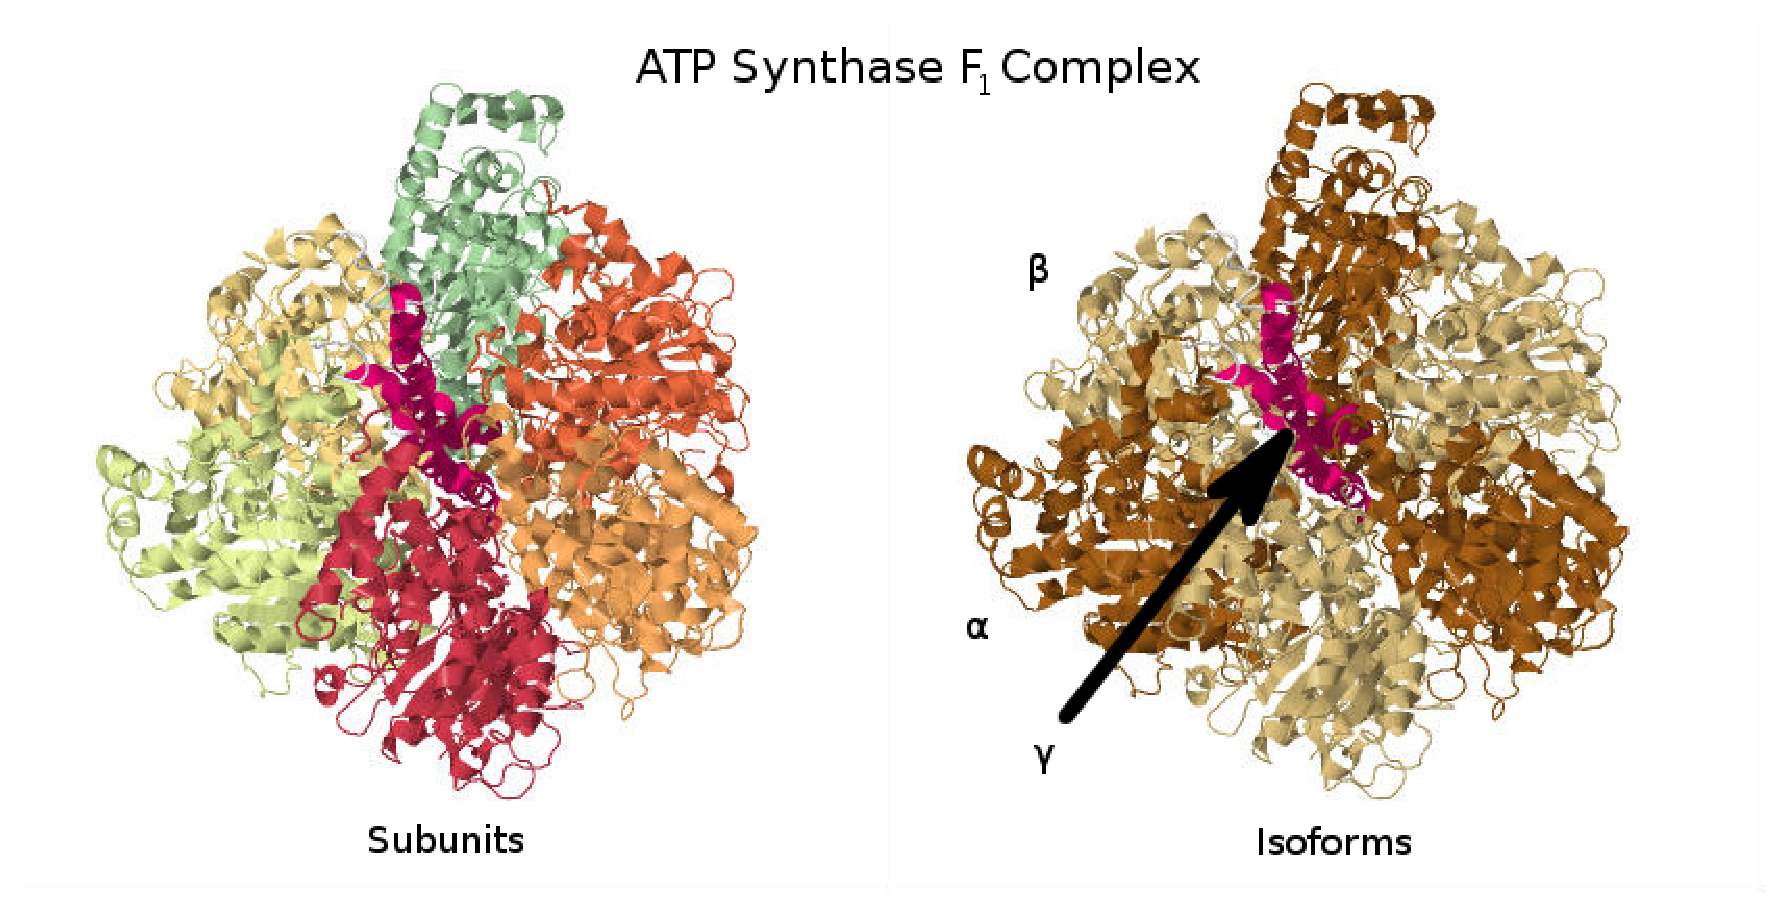
\includegraphics[clip=true,trim=0cm 0cm 0cm 0cm, width=12cm]{2F43}
\caption{Illustration of the $F_1$ part of the ATP Synthase complex
  (PDB ID 1E79; \citealt{Gibbons2000,Bernstein1978,Gezelter}).
  This illustration demonstrates both how an enzyme complex may be
  constituted by multiple subunits (left), and how some of those
  subunits may be products of the same gene and have differing
  stoichiometries within the complex (right).}
\label{fig:2F43}
\end{figure*}

\emph{Assumption~\ref{asm:hierarchy}.}
The modeling of enzyme complex abundance can be tackled by using
nested sets of subcomplexes; each enzyme complex consists of multiple
subcomplexes, unless it is only a single protein or family of protein
isozymes.  These subcomplexes are required for the enzyme complex to
function (AND relationships), and can be thought of as the division of
the complex in to distinct units that each have some necessary
function for the complex, with the exception that we do not keep track
of the multiplicity of subcomplexes within a complex since this
information is, in the current state of affairs, not always known.
However, there may be alternative versions of each functional set
(given by OR relationships). Eventually, this nested embedding
terminates with a single protein or set of peptide isoforms
(e.g.\ isozymes).  In the case of ATP Synthase, one of its functional
sets is represented by the $F_1$ subcomplex. The $F_1$ subcomplex
itself can be viewed as having two immediate subcomplexes: the single
$\gamma$ (axle) subunit and three identical subcomplexes each made of
an $\alpha$ and $\beta$ subunit. Each $\alpha\beta$ pair works
together to bind ADP and catalyze the reaction \citep{Oster2003}. The
$\alpha\beta$ subcomplex itself then has two subcomplexes composed of
just an $\alpha$ subunit on the one hand and the $\beta$ subunit on
the other.  It is obvious that one of these base-level functional
subcomplexes (in this example, either $\gamma$ or $\alpha\beta$) will
be in most limited supply, and that it will best represent the overall
enzyme complex abundance (discounting the issues of multiplicity for
$\alpha\beta$, discussed above).

%
% Consider adding this as a Theorem/Proof:
%

The hierarchical structure just described, when written out in
Boolean, will give a rule in CNF (conjunctive normal form), or more
specifically (owing to the lack of negations), clausal normal form,
where a clause is a disjunction of literals (genes). This is because all
relations are ANDs (conjunctions), except possibly at the inner-most
subcomplexes that have alternative isoforms, which are expressed as
ORs (disjunctions). Since GPR rules alone only specify the
requirements for enzyme complex formation, we will see that not all
forms of Boolean rules are equally useful in evaluating the enzyme
complex abundance, but we have established the assumptions in
Table~\ref{tab:ECAssume} and an alternative and logically equivalent rule
\citep{Russell2009} under which we can estimate enzyme complex copy
number.

\begin{table}
\def \ECAssumeCap {Assumptions in GPR-based Enzyme Complex Formation}
\ifthenelse{\boolean{thesisStyle}}{
  \begin{center} % also adds a little needed vspace
  \begin{tabular}{| p{0.9\textwidth} |}
  \hline
  \textbf{Table ~\ref{tab:ECAssume}. \ECAssumeCap} \\
  \hline
  % I put this in to a separate file because formatting the table in different ways
% is difficult; it may even be better to have multiple versions of this table
% for different documents, but hopefully we can avoid such code duplication.

%Internal part of the table:

\begin{enumerate}
% This is really not related to GPR rules: 
%\ifthenelse{\boolean{thesisStyle}}{\item} {} \label{asm:mm}
%Fluxes in general strive to operate near the $V_{max}$ of the
%reaction, which is proportional to enzyme complex abundance.
\item \label{asm:expcorr}
Expression values are highly correlated with the copy numbers of their
corresponding peptide isoforms.
\item \label{asm:isozyme} 
Protein isoforms contributing to isozymes are considered part of the
same enzyme complex.
\item \label{asm:hierarchy}
Any enzyme complex can be described as a hierarchical subset of
(possibly redundant) subcomplexes; redundant subcomplexes, as
elaborated in (\ref{asm:nostoich}), are not currently modeled.
\item \label{asm:nostoich} 
Assume one copy of peptide per complex; exact isoform stoichiometry
is not considered.
\item \label{asm:sharing} 
With the exception of complexes having identical rules (i.e. the same
complex listed for different reactions), each copy of a peptide
is available for all complexes in the model.
\item \label{asm:active_site}
There is only one active site per enzyme complex.
\item \label{asm:enzyme_sensitivity} 
We assume that different pathways have similar flux sensitivities
with respect to their enzyme abundances.
\item \label{asm:holo} 
If a particular subcomplex can be catalyzed by A and it can also be
catalyzed by A and B (e.g. B acts as a regulatory unit, as in
holoenzymes), this just simplifies to A once expression values are
substituted in. Similarly, allosteric regulation is not
modeled. Relatedly, there are no NOT operations in GPR rules (just ANDs
and ORs).
\item \label{asm:chap} 
Enzyme complexes form without the assistance of protein chaperones and
formation is not coupled to other reactions.
\item \label{asm:posttrans}
Post-translational modifications do not affect complex formation.
\item \label{asm:rate} 
Rate of formation and degradation of complexes doesn't play a role,
since we assume steady-state. 
\end{enumerate}

  \\ \hline
  \end{tabular}
  \end{center}

} {
  % For Bioinformatics:
  %\begin{table*}[!t]
  \processtable{\ECAssumeCap \label{tab:ECAssume}}{
  \begin{tabular}{| p{\textwidth} |}
  \hline
  % I put this in to a separate file because formatting the table in different ways
% is difficult; it may even be better to have multiple versions of this table
% for different documents, but hopefully we can avoid such code duplication.

%Internal part of the table:

\begin{enumerate}
% This is really not related to GPR rules: 
%\ifthenelse{\boolean{thesisStyle}}{\item} {} \label{asm:mm}
%Fluxes in general strive to operate near the $V_{max}$ of the
%reaction, which is proportional to enzyme complex abundance.
\item \label{asm:expcorr}
Expression values are highly correlated with the copy numbers of their
corresponding peptide isoforms.
\item \label{asm:isozyme} 
Protein isoforms contributing to isozymes are considered part of the
same enzyme complex.
\item \label{asm:hierarchy}
Any enzyme complex can be described as a hierarchical subset of
(possibly redundant) subcomplexes; redundant subcomplexes, as
elaborated in (\ref{asm:nostoich}), are not currently modeled.
\item \label{asm:nostoich} 
Assume one copy of peptide per complex; exact isoform stoichiometry
is not considered.
\item \label{asm:sharing} 
With the exception of complexes having identical rules (i.e. the same
complex listed for different reactions), each copy of a peptide
is available for all complexes in the model.
\item \label{asm:active_site}
There is only one active site per enzyme complex.
\item \label{asm:enzyme_sensitivity} 
We assume that different pathways have similar flux sensitivities
with respect to their enzyme abundances.
\item \label{asm:holo} 
If a particular subcomplex can be catalyzed by A and it can also be
catalyzed by A and B (e.g. B acts as a regulatory unit, as in
holoenzymes), this just simplifies to A once expression values are
substituted in. Similarly, allosteric regulation is not
modeled. Relatedly, there are no NOT operations in GPR rules (just ANDs
and ORs).
\item \label{asm:chap} 
Enzyme complexes form without the assistance of protein chaperones and
formation is not coupled to other reactions.
\item \label{asm:posttrans}
Post-translational modifications do not affect complex formation.
\item \label{asm:rate} 
Rate of formation and degradation of complexes doesn't play a role,
since we assume steady-state. 
\end{enumerate}

  \\ \hline
  \end{tabular}
  }
  {} % caption
}
\caption{A list of assumptions about how Gene-Protein-Reaction rules 
can describe enzyme complex stoichiometry.}
\label{tab:ECAssume}
\end{table}

There is no guarantee that a GPR rule has been written down with this
hierarchical structure in mind, though it is likely the case much of
the time as it is a natural way to model complexes.  However, any GPR
rule can be interpreted in the context of this hierarchical view due
to the existence of a logically equivalent CNF rule for any non-CNF
rule, and it is obvious that logical equivalence is all that is
required to check for enzyme complex formation when exact isoform
stoichiometry is unknown.  As an example, we consider another common
formulation for GPR rules, and a way to think about enzyme
structure---disjunctive normal form (DNF).  A DNF rule is a
disjunctive list of conjunctions of peptide isoforms, where each
conjunction is some variation of the enzyme complex due to
substituting in different isoforms for some of the required
subunits. A rule with a more complicated structure and compatible
isoforms across subcomplexes may be written more succinctly in CNF,
whereas a rule with only very few alternatives derived from isoform
variants may be represented clearly with DNF.  In rare cases, it is
possible that a GPR rule is written in neither DNF or CNF, perhaps
because neither of these two alternatives above are strictly the case,
and some other rule is more succinct.

\emph{Assumptions~\ref{asm:nostoich},~\ref{asm:sharing}~and~\ref{asm:active_site}.}
One active site per enzyme complex implies a single complex can only
catalyze one reaction at a time. Multimeric complexes with one active
site per identical subunit would be considered as one enzyme complex
per subunit in this model. Note that it is possible for an enzyme
complex to catalyze different reactions. In fact, some transporter
complexes can transfer many different metabolites across a lipid
bilayer---up to 294 distinct reactions in the reversible model for
solute carrier family 7 (Gene ID 9057).  Another example is the
ligation or hydrolysis of nucleotide, fatty acid, or peptide chains,
where chains of different length may all be substrates or products of
the same enzyme complex. While we do not explicitly consider these in
Algorithm~\ref{alg:ReductionToCNF}, these redundancies are taken into
account subsequently in Algorithm~\ref{alg:FALCON}.

What is currently not considered in our process is that some peptide
isoforms may find use in completely different complexes, and in some
cases, individual peptides may have multiple active sites; in the
first case, we assume an unrealistic case of superposition where the
isoform can simultaneously function in more than one complex. The
primary reason we have not tackled this problem is because exact
subunit stoichiometry of most enzyme complexes is not accurately
known, but an increasing abundance of data on BRENDA
\citep{Schomburg2013} gives some hope to this problem. A recent
\textit{E. coli} metabolic model incorporating the metabolism of all
known gene products \citep{O'Brien2013} also includes putative
enzyme complex stoichiometry in GPR rules. For the second point, there
are a few enzymes where a single polypeptide may have multiple active
sites (e.g.\ fatty acid synthase), and this is not currently taken into
account in our model. 

\emph{Assumption~\ref{asm:holo}.}
We do not make any special assumptions requiring symmetry of an
isoform within a complex. For instance, the example in
assumption~\ref{asm:holo} shows how you might have one subcomponent
composed of a single isoform, and another subcomponent composed of
that gene in addition to another isoform. In this case, it is simply
reduced to being the first gene only that is required, since clearly
the second is strictly optional. That isn't to say that the second
gene may not have some effect, such as (potentially) aiding in
structural ability or altering the catalytic rate, but it should have
no bearing on the formation of a functional catalytic
complex. Holoenzymes---enzymes with metabolic cofactors or protein
subunits that have a regulatory function for the complex---would
likely be the only situation where this type of rule might need to be
considered in more detail. But in the absence of detailed kinetic
information, this consideration (much like allosteric
regulation) is not useful.

\emph{Assumption~\ref{asm:enzyme_sensitivity}.}
Another important biochemical assumption is that reactions should
operate in a regime where they are sensitive to changes in the overall
enzyme level in the pathways that they belong in
\citep{Bennett2009,Chubukov2013}. This is perhaps the most important
issue to be explored further for methods like this, since if it is not
true, some other adjustment factor would be needed to make the method
realistic. For instance, if all reactions in a pathway are operating
far below $V_{max}$, but it is not the case in another pathway, the
current method does not have information on this, and will try to put
more flux through the first pathway than should be the case.

\emph{Assumptions~\ref{asm:chap}~and~\ref{asm:rate}.}
Due to the quickness, stability, and energetic favorability of enzyme
complex formation, the absence of chaperones or coupled metabolic
reactions required for complex formation may be reasonable
assumptions, but further research is warranted \citep{Karr2012}.
Additionally, as in metabolism, we assume a steady state for complex
formation, so that rate laws regarding complex formation aren't
needed. However, further research may be warranted to investigate the
use of a penalty for complex levels based on mass action and
protein-docking information. Requisite to this would be addressing
assumption~\ref{asm:nostoich}. It would be surprising (but not
impossible) if such a penalty were very large due to the cost this
would imply for many of the large and important enzyme complexes
present in all organisms \citep{Nelson2008}.

\section{The min-disjunction heuristic algorithm}
\label{sec:HeuristicToCNF}
Because conversion to CNF is potentially computationally intractable 
for some rules due to an  exponential increase in memory \citep{Russell2009}, we
present below a reduction rule that makes use of expression data.
The algorithm can be described as follows:

% TODO: write a function op commpand for M
\begin{algorithm} 
\caption{heuristic min disjunction}
\label{alg:HeuristicToCNF}
\begin{algorithmic}
\ifthenelse{\boolean{thesisStyle}}{\singlespacing}{}
\INPUT $G = \left\{g_i~\mid~i \in{1, \ldots, m}\right\}$ are genes. 
\INPUT $r$ := A Boolean rule without negation consisting of\\
  $\left\{x_i~\mid~i \in{1, \ldots, n}\right\}$ Boolean sub-expressions.
\INPUT $\E{g}$ := A map returning the expression level of gene g.
\While{$rule \neq o_1 \land \ldots \land o_p$ where each $o_i$ is a disjunction
  of genes} 
  \If {Encounter a disjunction $x_d$ of conjunctions of genes}
  \State \parbox[t]{\dimexpr\linewidth-\algorithmicindent}{
    Create sets from conjunctions, i.e.:\\
    Create $G_1$ and $G_2$ with $g_{1,i} \in G_1$ 
    and $g_{2,i} \in G_2$ where\\ 
    $x_d = (g_{1,1} \land \ldots \land g_{1,r}) \lor 
    (g_{2,1} \land \ldots \land g_{2,s})$. 
    \strut}
    \If {$G_1 \subseteq G_2$}
    \State Replace $x_d$ with $(g_{1,1} \land \ldots \land g_{1,r})$.
    \ElsIf {$G_2 \subseteq G_1$}
    \State Replace $x_d$ with $(g_{2,1} \land \ldots \land g_{2,s})$.
    \Else
    \State \parbox[t]{\dimexpr\linewidth-\algorithmicindent}{
      Create $G_C = G_1 \cap G_2$, \\
      $G_{1\setminus C} = G_1 \setminus G_C$ and\\ 
      $G_{2\setminus C} = G_2 \setminus G_C$. 
      \strut}
      \If {$G_{1\setminus C} = \varnothing\: ||\: G_{2\setminus C} = \varnothing$}
        \State Substitute $x_d$ with $\ANDw_{g_c \in G_C} g_c$.
      \Else
        \State \parbox[t]{\dimexpr\linewidth-\algorithmicindent}{Substitute $x_d$ with:\\
          $\ANDw_{g_c \in G_C} g_c \land (\mathcal{M}\left(G_{1 \setminus C}\right) \lor 
          \mathcal{M}\left(G_{2\setminus C}\right)$ where\\
          $\mathcal{M}\left(S\right) = \argmin_{g \in S}{\E{g}}$
          \strut}
      \EndIf
    \EndIf
  \EndIf
  \State \parbox[t]{\dimexpr\linewidth-\algorithmicindent}{
    Distribute $\lor$ over $\land$, e.g.: $(x_1 \land x_2) \lor (x_3 \land x_4)$ \\ 
    $\rightarrow (x_1 \lor x_3) \land (x_1 \lor x_4) \land 
    (x_2 \lor x_3) \land (x_2 \lor x_4)$
    \strut}
\EndWhile
\OUTPUT $o_{\min}$ where $o_{\min}$ has the form: $\ORw_{g_i \in G} g_i$
\end{algorithmic} 
\end{algorithm} 

The intuition for this algorithm is that it returns the minimum
disjunction because at each iteration; we select the literal with
smallest value in a conjunction and remove all other literals in the
conjunction. Distributing $\lor$ over $\land$ and subsequently
evaluating the associated expression values will not change which
disjunction attains the minimum value.

While this algorithm should work in most cases just as the algorithm
in Section~\ref{alg:ReductionToCNF}, there is a notable exception that
can occur when one or more genes appear in two conjunctions; this
possibility is handled in the conditional by treating the intersection
of the gene sets $G_C$ separately. Unfortunately, this step is not
associative over disjunctions, so if there are more than two
disjunctions at the same level, it is not guaranteed to be accurate.

While this algorithm is not currently implemented exactly as stated, 
an earlier version of this algorithm was implemented in ATS1, and
is available in the deprecated file \texttt{minDisjNoCov.dats}.
The algorithm can be implemented without much troubled based on the
existing code in the FALCON software package.

\subsection{Proof for the minDisjunction heuristic algorithm}

Although the intuition presented above may be straightforward, we show
here in more verbosity that Algorithm~\ref{alg:HeuristicToCNF} works
as described.

\begin{Theorem}
\label{thm:HeuristicToCNF}
Algorithm~\ref{alg:HeuristicToCNF} returns the disjunction with
minimum expression value among all disjunctions of a rule in CNF.
\end{Theorem}

\begin{proof}
Due to our Boolean algebra currently lacking negation, the only step
in converting to CNF that we need is the distributive expansion of 
$\land$ over $\lor$. However, in order to allow $\mathcal{M}$ to be
applied to conjunctive sets that are in disjunction with one another, 
we must ensure that the sets are disjoint, which is taken care of first
in the algorithm by handling the intersection of the conjunctive sets, 
$G_C = G_1 \cap G_2$, separately. In practice, if $G_{1\setminus C} = \varnothing$
or $G_{2\setminus C} = \varnothing$, then this means we have a situation similar
to that described in assumption~\ref{asm:holo}, and the entire expression
is simplified to $\ANDw_{g_c \in G_C} g_c$. Otherwise, a direct route is 
taken to compute distributive law for the literals: 

$\ANDw_{g_c \in G_C} g_c \land \left(\ANDw_{g_i \in G_{1 \setminus C}, 
g_j \in G_{2\setminus C}} \left(g_i \lor g_j\right) \right)$

Below, we show that by applying $\mathcal{M}$ to $G_{1\setminus C}$
and $G_{2\setminus C}$, we can compute the correct minimum
disjunction without the need to compute and store in memory every 
disjunction in the expansion, which results in the following:

$\ANDw_{g_c \in G_C} g_c \land \left(\mathcal{M}(G_{1 \setminus C}) 
\lor \mathcal{M}\left(G_{2\setminus C}\right)\right)$

Now let us consider when expressions $x_1, ..., x_4$
are all distinct literals, and that
$\E{x_i}$ denotes the enzyme abundance for expression $x_i$ (or the 
expression measure of $x_i$ if $x_i$ is a gene). Assume
WLOG that $x_1 \lor x_3$ attains the minimum expression among the
disjunctions. Then we have:

\begin{align*}
&\E{x_1} + \E{x_3} \leq \E{x_1} + \E{x_4} \Rightarrow \E{x_3} \leq \E{x_4} \\
&\E{x_1} + \E{x_3} \leq \E{x_2} + \E{x_3} \Rightarrow \E{x_1} \leq \E{x_2} 
\end{align*}

Applying this result in conjunction to the application of $\mathcal{M}$ to
the original expression, $(x_1 \land x_2) \lor (x_3 \land x_4)$, we
immediately arrive at $(x_1) \lor (x_3)$, which gives our originally
assumed minimum. To show that this result doesn't depend on the $x_i$
being literals, merely consider repeating this process recursively for
each $x_i$ that is not a literal to arrive at two different
evaluations for $\E{x_i}$ (one where each evaluation is done with
reduction, and one where we evaluate entirely without reduction).
Since the process cannot continue indefinitely, eventually there is a
base case involving only literals, and the above result shows that, at
each step, as we backtrack from the base case, both evaluations will
be identical. The desired result is obtained because
Algorithm~\ref{alg:HeuristicToCNF} without the conditional simply yields CNF,
and it follows that adding the conditional will yield the disjunction with
minimum expression value of the rule in CNF.
\end{proof}


\section{Generation of figures and tables}

All non-trivial figures can be generated using MATLAB scripts found in
the \texttt{analysis/figures} subdirectory of the FALCON installation.
In particular, figures should be generated through the master script
\texttt{makeMethodFigures.m} by calling
\texttt{makeMethodFigures(figName)} where \texttt{figName} has a name
corresponding to the desired figure.  In some cases, some MATLAB
\texttt{.mat} files will need to be generated by other scripts first;
see the plotting scripts or the subsections below for details. An
example is to make the scatter plots showing the difference between
running falcon with enzyme abundances determined by direct evaluation
or the minimum disjunction algorithm; all three scatter plots are
generated with the command \texttt{makeMethodFigures(\textquotesingle
fluxCmpScatter\textquotesingle)}. Note that, as written, this requires
a graphical MATLAB session.

Comparison of the effects of the employed enzyme complexation methods
were evaluated using \texttt{compareEnzymeExpression.m} and 
\texttt{compareFluxByRGroup.m}. Comparison of reacion groups was
performed in \texttt{compareFluxByRGroup.m}.

\subsection{Timing analyses}
All timing analyses were performed on a system with four 8-core AMD
Opteron\texttrademark\ 6136 processors operating at 2.4 GHz. Figure
FluxBars and Table FalcPerf used unperturbed expression data; see
\texttt{yeastResults.m} for details). Values for the FALCON method
were averaged across 32 replicates, while values for the
\citealt{Lee2012} method were averaged across 8 replicates. Human
timing analyses were performed using \texttt{methodTimer.m} with
8 replicates.

\subsection{Data sources}
Enzyme complexation comparisons were performed on proteomics data
from \citealt{Gholami2013} (Human; 786-O cell line) and 
\citealt{Picotti2013} (Yeast; BY strain), and on RNA-Seq data
from \citealt{Lee2012} (Yeast; 75\% max $\mu$ condition).